\hypertarget{a00337}{}\section{Plug-\/in meters}
\label{a00337}\index{Plug-\/in meters@{Plug-\/in meters}}
How to manage metering data for A\+A\+X plug-\/ins. 

\hypertarget{a00337_AdditionalFeatures_Meters_overview}{}\subsection{Overview of metering in A\+A\+X}\label{a00337_AdditionalFeatures_Meters_overview}
A\+A\+X provides a host-\/managed metering system for plug-\/ins. The host buffers, thins, and applies ballistics to each of the plug-\/in\textquotesingle{}s meters. When the plug-\/in G\+U\+I retrieves this processed data, it receives the exact same information that is displayed on control surfaces and other metering devices.\hypertarget{a00337_AdditionalFeatures_Meters_adding}{}\subsection{Adding meters to an Effect}\label{a00337_AdditionalFeatures_Meters_adding}
Meters are added to an algorithm Component in \hyperlink{a00326}{Describe} using \hyperlink{a00088_a5e4a61afa3d6510891e16d7179bdaa64}{A\+A\+X\+\_\+\+I\+Component\+Descriptor\+::\+Add\+Meters()}. The resulting meter context field will be populated with an array of meter \char`\"{}tap\char`\"{} values, one for each of the Component\textquotesingle{}s meters.\hypertarget{a00337_AdditionalFeatures_Meters_adding_properties}{}\subsubsection{Customizing meter behavior}\label{a00337_AdditionalFeatures_Meters_adding_properties}
Using the \hyperlink{a00096}{Effect Descriptor}, each meter in the Effect may optionally be associated with a \hyperlink{a00112}{property map} that applies a particular set of display properties to the meter. These are the properties that may be set on a meter\+:

\begin{DoxyItemize}
\item \hyperlink{a00206_af260f0f9a6bff0f7bfd3200b2947c96b}{A\+A\+X\+\_\+\+E\+Meter\+Orientation} \item \hyperlink{a00206_a9aaedbe356691c4e4584fa7ccdbcc776}{A\+A\+X\+\_\+\+E\+Meter\+Ballistic\+Type} \item \hyperlink{a00206_a590815545eaf0d3be0bb8f656fe2a761}{A\+A\+X\+\_\+\+E\+Meter\+Type}\end{DoxyItemize}
Note that, because meter properties are added at the Effect level, it is not possible to describe different meter property configurations for different algorithms in the same Effect.\hypertarget{a00337_AdditionalFeatures_Meters_reporting}{}\subsection{Reporting meter values}\label{a00337_AdditionalFeatures_Meters_reporting}
Meter values are reported by the algorithm using one \char`\"{}tap\char`\"{} per channel per buffer. For each tap, the algorithm must report the maximum metered sample value for each processing buffer.

Meter tap values can be interpreted as the maximum value of the meter per buffer, on a scale of \mbox{[}0.\+0 1.\+0\mbox{]}. In all cases the plug-\/in\textquotesingle{}s meter position should be normalized between 0 and 1, where 0 is no gain reduction. For example\+:

\begin{DoxyItemize}
\item An input meter should report the maximum absolute sample value that is present in the input audio buffer for the appropriate channel \item An output meter should report the maximum absolute sample value that is present in the output audio buffer for the appropriate channel \item A gain-\/reduction meter (C\+L or E\+G types) should report the largest amount of gain reduction in the current buffer for the appropriate channel. If no gain reduction occurred for a buffer then a value of 0.\+0 should be reported. If a full-\/scale signal was reduced to silence then a value of 1.\+0 should be reported.\end{DoxyItemize}
Gain-\/reduction meter values should report peak gain reduction, not R\+M\+S or other algorithms, and may use any normalization mapping (e.\+g. linear, exponential) which is desired. Ideally the gain-\/reduction metering U\+I in the host and on attached control surfaces will match the Peak gain redution metering in the plug-\/in\textquotesingle{}s G\+U\+I.

\begin{DoxyRefDesc}{Legacy Porting Notes}
\item[\hyperlink{a00384__porting_notes000001}{Legacy Porting Notes}]The gain-\/reduction meter handling for A\+A\+X plug-\/ins is different from that for R\+T\+A\+S/\+T\+D\+M plug-\/ins. A\+A\+X plug-\/ins must invert their gain-\/reduction meter values manually before reporting these values from the audio processing callback. The A\+A\+X host will always thin reported meter data using a \char`\"{}max\char`\"{} operation, and will later invert gain-\/reduction meter values before they are available to the plug-\/in G\+U\+I or to control surfaces. \end{DoxyRefDesc}
\hypertarget{a00337_AdditionalFeatures_Meters_displaying}{}\subsection{Displaying meter values}\label{a00337_AdditionalFeatures_Meters_displaying}
The meter values that are reported to the system from the algorithm are available, in buffered and (optionally) ballistics-\/smoothed form, from \hyperlink{a00090}{A\+A\+X\+\_\+\+I\+Controller} . The meter values returned from methods such as \hyperlink{a00090_a13de9cc4bb7fb3848fbe12622c033135}{Get\+Current\+Meter\+Value()} and \hyperlink{a00090_a85db3824256005c97689925750103765}{Get\+Meter\+Peak\+Value()} are the same values used by the system when displaying plug-\/in meters on control surfaces, and when a plug-\/in clears the peak value using \hyperlink{a00090_aa8fe057d2f53109e75662da0a492fa34}{Clear\+Meter\+Peak\+Value()} this change will likewise be reflected throughout the system.

The literal values provided by these methods can be interpreted as the distance from \char`\"{}rest\char`\"{} that the meter must travel to represent the current value, again on a scale of \mbox{[}0.\+0 1.\+0\mbox{]}. Note that this is not necessarily equivalent to the semantics of the meter\textquotesingle{}s reported values in the algorithm\+:

\begin{DoxyItemize}
\item For \char`\"{}standard\char`\"{} meters such as input meters, this corresponds to the value provided by the algorithm, since a maximum metered sample value (1.\+0) corresponds to a meter that should be drawn \char`\"{}furthest from rest\char`\"{} (1.\+0), i.\+e. at the top of a standard bottom-\/to-\/top meter graphic, or at the far right of a standard left-\/to-\/right graphic. \item For \char`\"{}inverted\char`\"{} meters, such as gain-\/reduction meters, these semantics are reversed\+: a maximum metered sample value (1.\+0) corresponds to a meter drawn \char`\"{}at rest\char`\"{} (0.\+0), i.\+e. at the bottom of a bottom-\/to-\/top meter graphic or at the far left of a left-\/to-\/right graphic.\end{DoxyItemize}
These values are independent of \hyperlink{a00206_af260f0f9a6bff0f7bfd3200b2947c96b}{meter orientation}\+: an input or output meter that is oriented with \hyperlink{a00206_af260f0f9a6bff0f7bfd3200b2947c96ba0b672f16509ea26e7374306bbb2e1e07}{A\+A\+X\+\_\+e\+Meter\+Orientation\+\_\+\+Top\+Right} will still use 0.\+0 as its \char`\"{}at rest\char`\"{} position, and likewise a gain-\/reduction meter that is oriented with \hyperlink{a00206_af260f0f9a6bff0f7bfd3200b2947c96bad6b506082c761babe2cefe133d326e32}{A\+A\+X\+\_\+e\+Meter\+Orientation\+\_\+\+Bottom\+Left} will still use 1.\+0.\hypertarget{a00337_AdditionalFeatures_Meters_alternatives}{}\subsection{Alternatives}\label{a00337_AdditionalFeatures_Meters_alternatives}
For advanced metering applications a single tap value may not be sufficient. To transmit more detailed information from the algorithm to its other components, a plug-\/in must use the \hyperlink{a00333}{Direct Data} interface. Collaboration diagram for Plug-\/in meters\+:
\nopagebreak
\begin{figure}[H]
\begin{center}
\leavevmode
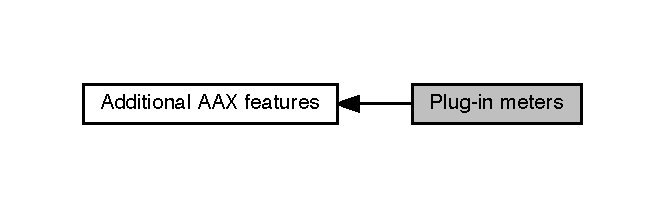
\includegraphics[width=319pt]{a00337}
\end{center}
\end{figure}
